\title{CS534 Implementation Assignment 3:\\Bagging and AdaBoost}
\author{
        Amit Bawaskar, Michael Lam\\
        EECS, Oregon State University\\
        %\email{}
        %\and
}

\documentclass[12pt]{article}
\usepackage[english]{babel}
\usepackage{graphicx}
\usepackage{subfig}
\usepackage{amsmath}
\usepackage{hyperref}
\hypersetup{
    colorlinks,%
    citecolor=green,%
    filecolor=magenta,%
    linkcolor=red,%
    urlcolor=cyan
}

%\underset{x}{\operatorname{argmax}}
%\underset{x}{\operatorname{argmin}}
\DeclareMathOperator*{\argmin}{arg\,min}
\DeclareMathOperator*{\argmax}{arg\,max}

\begin{document}
\maketitle

\begin{abstract}
In this assignment we implemented and evaluated bagging and AdaBoost using the decision stump as the base learner.
\end{abstract}

% -------------------------------------------------
\section{Introduction}
Ensemble methods such as bagging and AdaBoost work by taking a base learner and generating a set (ensemble) of hypotheses by varying the training set. The final hypothesis for classification is a majority vote of these hypotheses. The decision stump is a suitable base learner for bagging and especially AdaBoost because it is a weak learner, meaning it classifies slightly better than random.

In this assignment we implemented the decision stump, bagging and AdaBoost. For each ensemble method we evaluated the training and test errors as a function of the ensemble size.

\section{Decision Stump}
The decision stump is a one level decision tree. In this assignment all features and labels are binary. Therefore the decision stump is a one level binary tree with a binary feature test at the root node connected to two leaf nodes each containing a label.

Learning is done by going through every feature in the training data and computing the maximum information gain (minimum entropy). Once the feature with the maximum information gain is determined, the two leaf nodes are given the label of the majority class from splitting the training data on that feature. Inference is done by simply testing the feature and assigning the label following the appropriate branch.

For AdaBoost, decision stump learning also accepts a distribution of the data as input. Therefore each training example is weighted differently based on the distribution, which affects the information gain computation and leaf node labels in every iteration of AdaBoost.

\section{Bagging}
Explain bagging and how we implemented

\section{AdaBoost}
Boosting is an ensemble method that considers errors from previous hypotheses to decide how to sample the training data for the next iteration. This is in contrast to bagging, which individual classifiers were independent. Boosting works when the base learner is weak learner, i.e. its classification accuracy is slightly better than random.

AdaBoost is a particular boosting algorithm that maintains and updates a distribution over the training data based on the hypothesis error at each iteration. Thus each training data point is given more or less weight according to the distribution \(D\). At each iteration \(t\) AdaBoost records the current hypothesis and a weight \(\alpha_t\) computed from the weighted error \(\epsilon_t\). The distribution \(D\) is updated using the computed \(\alpha_t\).

These equations are shown below, for \(m\) training examples \(x_i\) and their labels \(y_i\), distribution \(D_t(i)\) at time \(t\) for \(i\)th example, hypothesis \(h_t\) from weak base learner (i.e. decision stump) at time \(t\) and \(Z\) is a normalization factor to make \(D_{t+1}\) a distribution:

\begin{align}
 \epsilon_t = \sum_{i=1}^{m} D_t(i) I(y_i \neq h_t(x_i)) \\
 \alpha_t = \frac{1}{2} log\left(\frac{1-\epsilon_t}{\epsilon_t}\right) \\
 D_{t+1}(i) = \frac{ D_{t}(i)exp(-\alpha_t y_i h_t(x_i)) }{Z} & & \forall i = 1,...,m \\
\end{align}

The final hypothesis is just the sign of the weighted sum of each hypothesis and its corresponding weight \(\alpha\).

\section{Results}
For AdaBoost, figure \ref{fig:adaboost_trainerrors} plots the training errors versus the ensemble size, and figure \ref{fig:adaboost_testerrors} plots the test errors versus the ensemble size.

\begin{figure}[!t]
  \centering
  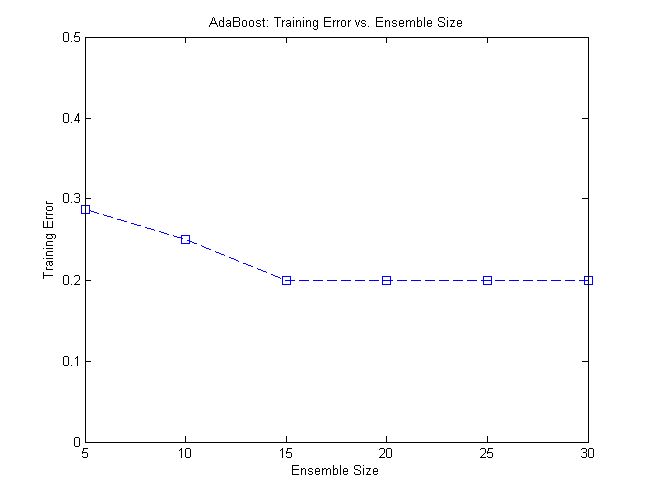
\includegraphics[scale=.75]{img/adaboost_trainerrors.png}
  \caption{AdaBoost training errors on different ensemble sizes.}
  \label{fig:adaboost_trainerrors}
\end{figure}

\begin{figure}[!t]
  \centering
  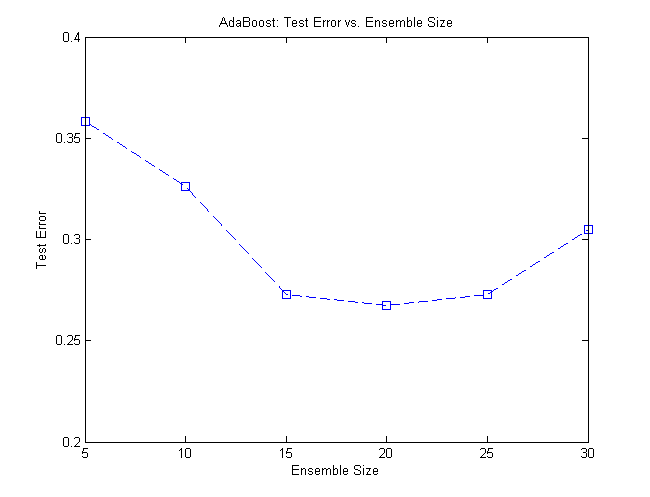
\includegraphics[scale=.75]{img/adaboost_testerrors.png}
  \caption{AdaBoost test errors on different ensemble sizes.}
  \label{fig:adaboost_testerrors}
\end{figure}

\section{Discussion}
For AdaBoost, the training error appears to decrease as the ensemble size increases but then flattens out at ensemble size 15 and greater for the given training data. This indicates that while AdaBoost continues to select new hypotheses and weights (otherwise it would terminate), the training error does not improve. Interestingly, from observing the ensemble of hypotheses for ensemble size 30, there is a brief period after iteration 15 where the decision stump uses feature 17 iteration after iteration with more or less similar weights but with different leaf node labels. This may explain why the training error doesn't improve; the hypotheses and weights after iteration 15 have negligible impact on the final classifier.

The AdaBoost test (generalization) error decreases and performs the best at around ensemble size 20, but then increases afterward. This trend is typical of test curves in machine learning; it indicates that test error decreases with the training error but eventually increases due to over fitting.

%\begin{align}
% 1+1=2
%\end{align}
%
%Figure \ref{fig:example} is an example.
%
%\begin{figure}[!t]
%  \centering
%  \includegraphics[scale=1]{img/example.png}
%  \caption{Caption example.}
%  \label{fig:example}
%\end{figure}

\end{document}
This is never printed
